\documentclass{beamer}
\usetheme[pageofpages=de,% String used between the current page and the
                         % total page count.
          bullet=circle,% Use circles instead of squares for bullets.
          titleline=true,% Show a line below the frame title.
          alternativetitlepage=true,% Use the fancy title page.
          titlepagelogo=../img/fse_ministerio_ancho_texto.png%,% Logo for the first page.
	  %watermark=junta_girado,
          %watermarkheight=75px,% Height of the watermark.
          %watermarkheightmult=4,% The watermark image is 4 times bigger
                                % than watermarkheight.
          ]{Torino}

\usepackage[spanish]{babel} % Para separar correctamente las palabras
\usepackage[utf8]{inputenc} % Este paquete permite poner acentos y eñes usando codificación utf-8

\usepackage{color}

\author{
\small{IES Gonzalo Nazareno}\\
\tiny{Dos Hermanas (Sevilla)}\\
\small{IES Los Albares}\\
\tiny{Cieza (Murcia)}\\
\small{IES La Campiña}\\
\tiny{Arahal (Sevilla)}\\
\small{IES Ingeniero de la Cierva}\\
\tiny{Murcia}\\
\vspace{.5cm}

\includegraphics[width=0.2\textwidth]{cc_by_sa.png}}
\title{Introducción a OpenStack}
\institute{Proyecto de Innovación\\ {\color{white} .\\} \emph{Implantación y
    puesta a punto de la infraestructura de un cloud computing privado para el
    despliegue de servicios en la nube}}  

\begin{document}
\setlength{\parskip}{.2cm}

\begin{frame}[t,plain]
\titlepage
\end{frame}

\begin{frame}
  \frametitle{Cloud Computing}
  Pequeña intro.
\end{frame}

\begin{frame}
  \frametitle{Cloud Computing}
  Tradicionalmente se definen tres capas:
  \begin{description}
  \item[Software as a Service (SaaS)] Aplicación completa ofrecida
    como servicio en la nube (Servicios de Google, Salesforce.com, Microsoft
    Office 365, \ldots)
  \item[Platform as a Service (PaaS)] Aplicación completa para el
    desarrollo ofrecida como servicio en la nube (Google App Engine,
    Windows Azure, RedHat OpenShift, \ldots)
  \item[Infrastructure as a Service (IaaS)] Almacenamiento (también
    denominado \textit{Storage as a Service}) y capacidades de cómputo
    (máquinas completas) ofrecida como servicio en la nube.
  \end{description}
\end{frame}

\begin{frame}
  \frametitle{Tipos de IaaS}
  \begin{description}
  \item[Público] Una empresa ofrece IaaS a terceros, encargándose de
    toda la gestión del Cloud. El caso más conocido es Amazon Elastic
    Cloud Computing (EC2).
  \item[Privado] Una organización configura sus propios recursos como
    IaaS para tener más flexibilidad y control total sobre sus
    recursos.
  \item[Híbrido] Algunos servicios se gestionan en el cloud privado y
    otros se transfieren a uno público, normalmente utilizan una API
    común que permita una buena integración.
  \end{description}
\end{frame}

\begin{frame}
  \frametitle{Inicios de OpenStack}
  \begin{tabular}[center]{cl}
    
\includegraphics[width=.2\textwidth]{../img/rackspace.jpg}&
    \parbox{0.75\textwidth}{
      \begin{itemize}
      \item Cloud propio desde 2005
        \begin{itemize}
        \item Cloud servers (IaaS)
        \item Cloud files (StaaS)
        \end{itemize}
      \item Este software cambia a licencia libre en Abril 2010
      \end{itemize}}\\
    \hline
    
\includegraphics[width=.1\textwidth]{../img/nasa.png}&
    \parbox{.75\textwidth}{
      \begin{itemize}
      \item Comienza a utilizar Eucalyptus, pero lo descarta por no ser
        completamente libre (es ``open core'')
      \item Crea el software para IaaS Nebula
      \item Nebula cambia a licencia libre en Mayo 2010
      \end{itemize}}\\
    \hline
    
\includegraphics[width=.1\textwidth]{../img/openstack.jpg}&
    \parbox{.75\textwidth}{
      \begin{itemize}
      \item Nasa y Rackspace lo inician en Junio de 2010
      \item Dos componentes principales:
        \begin{itemize}
        \item OpenStack Compute (nova), deriva de Nebula
        \item OpenStack Object Store (swift), deriva de cloud files
        \end{itemize}
      \end{itemize}}\\
  \end{tabular}
\end{frame}

\begin{frame}
  \frametitle{Objetivo de OpenStack}
  \begin{center}
    ``Crear una plataforma en software libre para cloud computing que cumpla con
    las necesidades de los proveedores de nubes públicas y privadas,
    independientemente de su tamaño, que sea fácil de implementar y masivamente
    escalable.''
  \end{center}
\end{frame}

\begin{frame}
  \frametitle{Principios fundacionales de OpenStack}
  \begin{itemize}
  \item Licencia Apache 2.0, no existe versión ``enterprise''
  \item Proceso de diseño abierto
  \item Repositorios públicos de código fuente
  \item Todos los procesos de desarrollo deben estar documentados y ser
    transparentes
  \item Orientado para adoptar estándares abiertos
  \item Diseño modular que permite flexibilidad mediante el uso de APIs
  \end{itemize}
\end{frame}
\begin{frame}[fragile]
  \frametitle{OpenStack es libre}
  \begin{itemize}
  \item OpenStack es un proyecto con licencia libre (Apache)
  \item Diseño abierto:
    \begin{itemize}
    \item \url{http://blueprints.launchpad.net/openstack}
    \item \url{http://www.openstack.org/summit/san-diego-2012/}
    \end{itemize}
  \item Desarrollo abierto:
    \begin{itemize}
    \item \url{http://launchpad.net/openstack} y \url{http://github.com/openstack/}
    \item Lenguaje de programación Python
    \item \url{http://bugs.launchpad.net/openstack/}
    \end{itemize}
    \item Comunidad abierta:
      \begin{itemize}
      \item \url{http://www.openstack.org/community/}
      \item \url{http://www.openstack.org/foundation/companies/}
      \item \url{http://lists.openstack.org}
      \end{itemize}
    \item Comunidad + empresas
  \end{itemize}
\end{frame}

\begin{frame}
  \frametitle{Versiones de OpenStack}
  \begin{itemize}
  \item Proyecto muy nuevo, pero con un fuerte ritmo de desarrollo
    \begin{description}
    \item[Austin] 21 Octubre 2010
    \item[Bexar] 3 Febrero 2011
    \item[Cactus] 15 Abril 2011
    \item[Diablo] 22 Septiembre 2011 (Publicación semestral)
    \item[Essex] 5 Abril 2012
    \item[Folsom] 27 Septiembre 2012
    \item[Grizzly] Previsto 4 Abril 2013
    \end{description}
  \item Está previsto que se publiquen dos versiones al año
  \item Hasta ahora cada versión incluye importantes modificaciones respecto a
    la anterior
  \item Essex ha sido la primera versión ``completa''
  \item Desde Cactus, la publicación se ``acopla'' a la de Ubuntu
  \end{itemize}
\end{frame}

\begin{frame}[fragile]
  \frametitle{OpenStack Essex}
  \begin{itemize}
  \item Primera versión ``completa'' de OpenStack
  \item ¿Por qué es importante Essex?
    \begin{itemize}
    \item Presente en Ubuntu 12.04 LTS. La próxima versión LTS será en 2014
    \item Presente en Debian Wheezy (próxima estable). Debian wheezy soportará
      OpenStack Folsom en backport
    \end{itemize}
  \item Componentes de OpenStack Essex:
    \begin{itemize}
    \item OpenStack Compute (nova)
    \item OpenStack Object Store (swift)
    \item OpenStack Image (glance)
    \item OpenStack Identity (keystone) $\leftarrow$ Nuevo en Essex
    \item OpenStack Dashboard (horizon) $\leftarrow$ Nuevo en Essex
    \end{itemize}
  \end{itemize}
  \url{http://wiki.openstack.org/ReleaseNotes/Essex}
\end{frame}

\begin{frame}
  \frametitle{OpenStack Folsom}
  \begin{itemize}
  \item OpenStack tiene un ritmo de publicación semestral, difícil de incluir en
    la publicación de distribuciones ``estables''. Ubuntu LTS o Debian se
    publican cada dos años.
  \item Incluye mejoras en bastantes componentes de OpenStack
  \item Incluido en Ubuntu 12.10
  \item Se incluirá en Debian Wheezy mediante backport (repositorio extra menos
    estable)
  \item Las principales novedades son la aparición de dos nuevos componentes
    principales:
    \begin{itemize}
    \item OpenStack Network Service (Quantum)
    \item OpenStack Block Storage (Cinder)
    \end{itemize}
  \end{itemize}
  \url{http://wiki.openstack.org/ReleaseNotes/Folsom}
\end{frame}

\begin{frame}
  \frametitle{Servicios de OpenStack nova}
  \begin{itemize}
  \item Nova es el componente principal de OpenStack y está compuesto por varios
    servicios independientes:
    \begin{description}
    \item[nova-api] Encargado de aceptar las peticiones de los usuarios o del
      resto de componentes de OpenStack mediante una API RESTful
    \item[nova-scheduler] Encargado de planificar la ejecución de las instancias
      en los diferentes nodos del cloud
    \item[nova-compute] Encargado de ejecutar una instancia sobre un hipervisor
    \item[nova-network] Encargado de la comunicación de la instancia con el
      exterior
    \item[nova-volume] Encargado de gestionar los volúmenes asociados a las
      instancias (sustituido en Folsom por Cinder)
    \end{description}
  \item Los componentes de nova se comunican entre sí mediante AMQP
  \end{itemize}
\end{frame}

\begin{frame}
  \frametitle{Funcionamiento de OpenStack}
  \begin{itemize}
  \item Un usuario interactúa con la API de nova (bien directamente o
    indirectamente a través de horizon) para ejecutar una instancia.
  \item nova-api le pedirá que se autentique previamente con keystone
  \item Una vez autenticado le mostrará las imágenes disponibles en glance
  \item Cuando seleccione una imagen y unas características para la instancia,
    se enviará a nova-scheduler la petición
  \item Nova-scheduler determinará en que nodo debe ejecutarse la instancia
  \item Nova-compute del nodo seleccionado se encargará de ejecutar la instancia
    sobre el hipervisor que disponga
  \item Nova-network realizará las configuraciones necesarias en la red
  \item Nova-volume se encargará de gestionar en su caso los volúmenes asociados
    a la instancia
  \end{itemize}
\end{frame}

\begin{frame}
  \frametitle{Funcionamiento de OpenStack}
  \begin{center}
    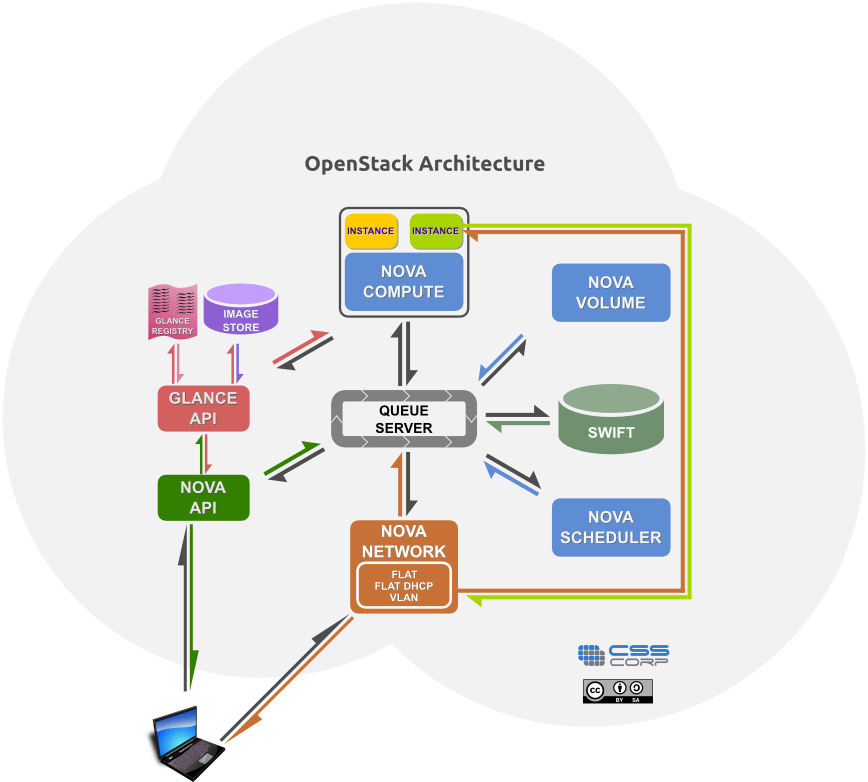
\includegraphics[height=.75\textheight]{../img/Archhtml.png}
  \end{center}
\end{frame}

\begin{frame}
  \frametitle{Instalación de componentes de OpenStack }
  \begin{itemize}
  \item Dependiendo del número de equipos del cloud y la configuración de red,
    se instalarán en cada nodo diferentes componentes, p. ej.:
  \end{itemize}
  \begin{center}
    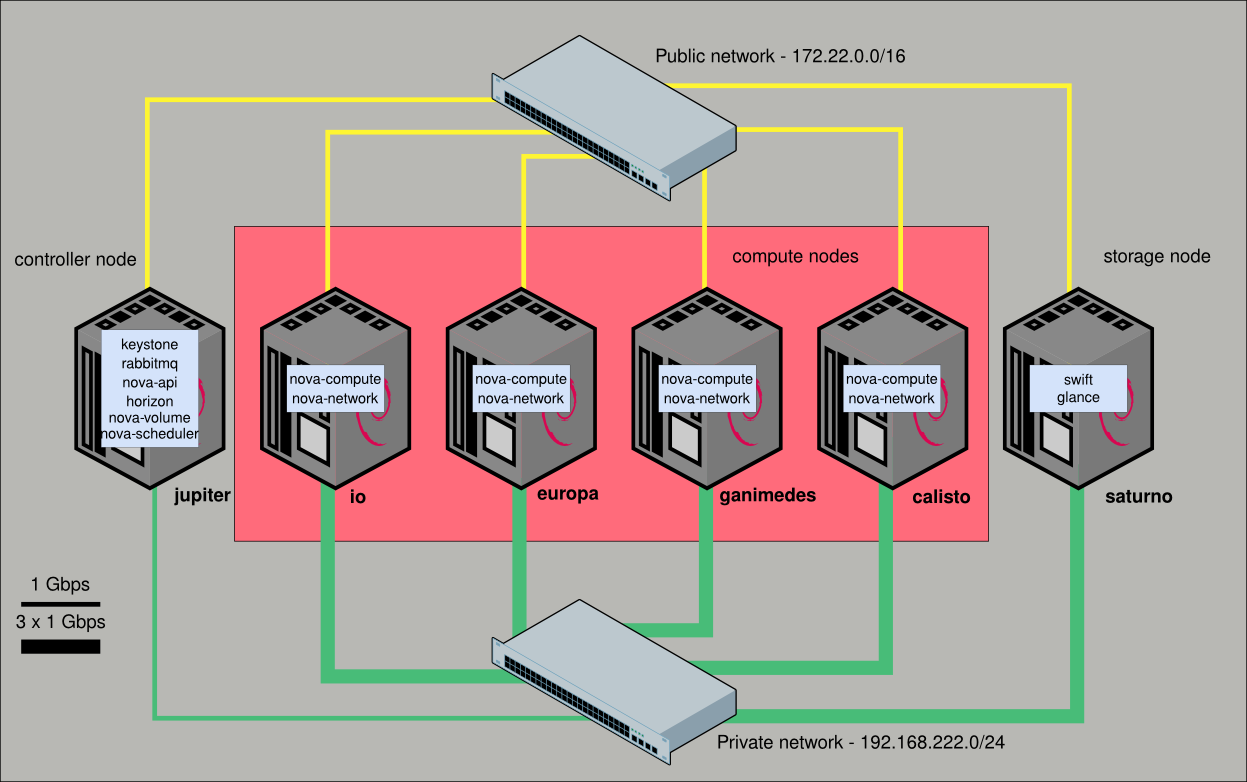
\includegraphics[width=.8\textwidth]{../img/esquema_red_iesgn}    
  \end{center}
\end{frame}
% \begin{frame}
%   \frametitle{OpenStack Folsom}
%   
% \end{frame}
% \begin{frame}
%   \frametitle{Cloud de infraestructura privado con software libre}
%   La mejor opción para utilizar en un entorno educativo es un cloud de
%   infraestructura privado basado en software libre
%   \begin{description}
%   \item[¿Por qué privado?] Permite control total sobre el cloud,
%     utilizarlo sin límites y conocerlo de forma detallada.
%   \item[¿Por qué libre?] Entre otros motivos:
%     \begin{itemize}
%     \item Permite control total sobre software
%     \item Garantiza la independencia tecnológica
%     \item Utiliza estándares
%     \item Interoperabilidad
%     \item Ahorro de costes
%     \end{itemize}
%   \end{description}
% Las dos opciones más interesantes actualmente son OpenStack y OpenNebula
% \end{frame}

% \begin{frame}
%   \frametitle{Evolución metodológica}
%   Antes de ver las posibilidades que ofrece la utilización de IaaS en las
%   enseñanzas de informática, vamos a recapitular las fases por las que han
%   pasado estas enseñanzas\footnote{Nos referimos siempre a enseñanzas prácticas,
%   no a la tiza ;)}
%   \begin{itemize}
%   \item A la par de la evolución tecnológica, se ha producido una evolución en
%     los métodos de enseñanza de informática, que podríamos de forma muy general
%     separar en 3 fases:
%     \begin{itemize}
%     \item Primera fase: Utilización de equipos físicos
%     \item Segunda fase: Utilización de máquinas virtuales
%     \item Tercera fase: Utilización de IaaS
%     \end{itemize}
%   \item Estas fases no son excluyentes: una fase siempre puede incluir las
%     anteriores.
%   \item Todas tienen ventajas e inconvenientes, pero la tercera fase ofrece
%     escenarios imposibles de utilizar anteriormente.

%   \end{itemize}
% \end{frame}

% \begin{frame}
%   \frametitle{Evolución metodológica. Primera fase}
%   \begin{columns}
%     \column{.6\textwidth}
%     \begin{itemize}
%     \item Utilización de máquinas físicas
%       \begin{itemize}
%       \item Una máquina por alumno
%       \item Algunos servidores compartidos
%       \end{itemize}
%       \item Pros:
%       \begin{itemize}
%       \item Fácil despliegue y puesta en marcha
%       \end{itemize}
%       \item Contras:
%       \begin{itemize}
%       \item Prácticas muy limitadas por número de equipos y tipo de
%         configuraciones
%       \item Hardware poco variado
%       \item Prácticas muy ``académicas''
%       \item Muchos tiempos muertos entre prácticas
%       \end{itemize}
%     \end{itemize}
%     \column{.4\textwidth}
%     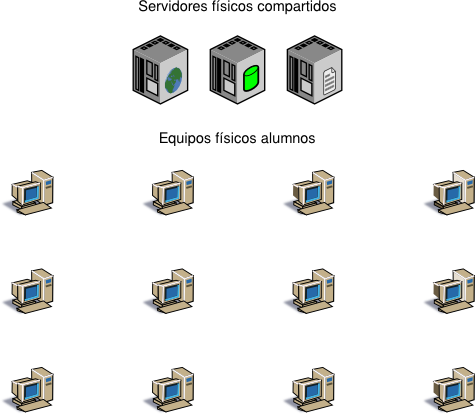
\includegraphics[width=\columnwidth]{../img/epoca1.png}
%   \end{columns}
% \end{frame}

% \begin{frame}
%   \frametitle{Evolución metodológica. Segunda fase}
%   \begin{columns}
%     \column{.6\textwidth}
%     \begin{itemize}
%     \item Utilización de máquinas virtuales
%       \begin{itemize}
%       \item Una máquina por alumno
%       \item Varias máquinas virtuales por máquina física
%       \end{itemize}
%       \item Pros:
%       \begin{itemize}
%       \item Cada alumno dispone de un entorno ``completo'' e independiente
%       \item Prácticas menos rígidas
%       \item Se aprende virtualización de forma transversal
%       \end{itemize}
%       \item Contras:
%       \begin{itemize}
%       \item Entorno más complejo
%       \item Requiere equipos actualizados para los alumnos
%       \item Los alumnos tienen que administrar el gestor de máquinas
%         virtuales 
%       \end{itemize}
%     \end{itemize}
%     \column{.4\textwidth}
%     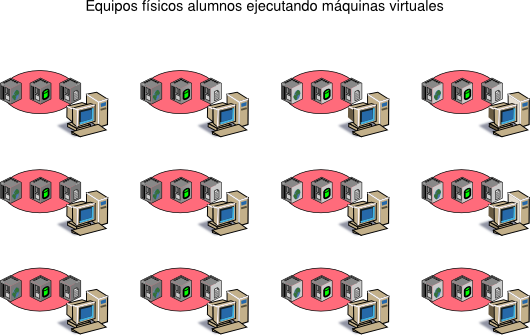
\includegraphics[width=\columnwidth]{../img/epoca2.png}
%   \end{columns}
% \end{frame}

% \begin{frame}
%   \frametitle{Evolución metodológica. Tercera fase}
%   \begin{columns}
%     \column{.6\textwidth}
%     \begin{itemize}
%     \item Utilización de IaaS
%       \begin{itemize}
%       \item Un equipo convencional por alumno
%       \item IaaS privado de la organización
%       \end{itemize}
%       \item Pros:
%       \begin{itemize}
%       \item Enorme variedad de prácticas
%       \item Utilización de entornos preconfigurados
%       \item Simulación de entornos reales complejos
%       \item Equipos básicos para los alumnos
%       \item Se aprende IaaS de forma transversal
%       \end{itemize}
%       \item Contras:
%       \begin{itemize}
%       \item Sistema muy centralizado
%       \item Imprescindible administración del Cloud
%       \item Inversión inicial importante
%       \end{itemize}
%     \end{itemize}
%     \column{.4\textwidth}
%     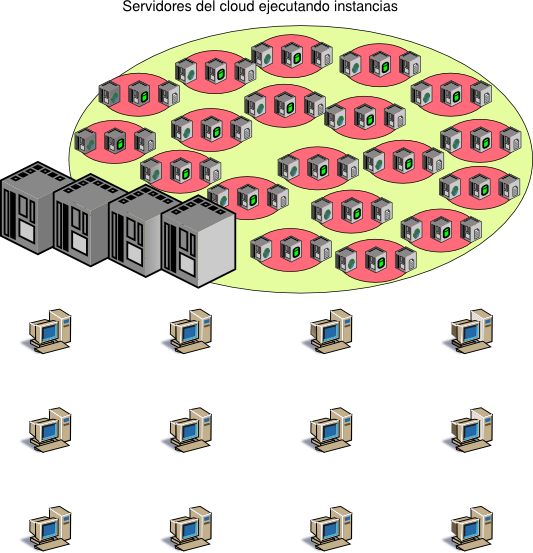
\includegraphics[width=\columnwidth]{../img/epoca3.png}
%   \end{columns}
% \end{frame}

% \begin{frame}
%   \frametitle{Simulación de entornos reales}
%   Un entorno real es difícil de simular con MVs en un PC por sus
%     propias limitaciones, pero en un cloud es asumible:
%     \begin{itemize}
%     \item Se puede simular una red con un número importante de equipos
%     \item Se puede utilizar la diversidad que se quiera de SOs
%     \item Este entorno ``real'' pueden utilizarlo conjuntamente todos los
%       alumnos
%     \item Puede estar disponible durante todo el curso sin interferir con otras
%       asignaturas
%     \item Con el tiempo y el uso irán apareciendo conflictos y problemas reales
%     \end{itemize}
% \end{frame}
% \begin{frame}
%   \frametitle{Nueva forma de aprendizaje}
%   \begin{itemize}
%   \item La utilización de IaaS en el ámbito académico conlleva una nueva forma
%     de aprender
%   \item Con el uso de MVs se había impuesto una forma de aprender que no era
%     siempre la mejor, por ejemplo:
%     \begin{itemize}
%     \item Para utilizar un SGBD había que instalarlo y configurarlo antes
%     \item Para desplegar una aplicación web, había que configurar previamente
%       todo el servidor de aplicaciones
%     \item Para hacer prácticas de ZFS había que instalar Solaris o FreeBSD
%     \end{itemize}
%     \item Un cloud puede contar con gran cantidad de imágenes preconfiguradas de
%       sistemas con muy diversas configuraciones $\Rightarrow$ La forma de
%       aprender no viene condicionada por la necesidad de una configuración
%       previa, por ejemplo:
%       \begin{itemize}
%       \item Primero se utiliza el SGBD durante varias clases.
%       \item Posteriormente, cuando sea oportuno, se aprende a instalarlo y
%         configurarlo
%       \end{itemize}
%   \end{itemize}
% \end{frame}

% \begin{frame}
%   \frametitle{Escenarios (I)}
%   \begin{description}
%   \item[Instalación y configuración de un servicio]
%   \end{description}
%   Los pasos típicos a seguir serían:
%   \begin{itemize}
%   \item Cada alumno inicia una instancia del SO en el que va a instalar el
%     servicio (no es necesario que previamente sepa instalar ese SO).
%   \item Realiza la instalación del servicio
%   \item Realiza la configuración del servicio. Si esta configuración dura
%     más de una clase, suspende la instancia y la reinicia en la siguiente
%     clase.
%   \item Una vez terminada la configuración puede crear una instantánea para
%     utilizarla como base en posteriores prácticas.
%   \item Si algún alumno no ha podido realizar la configuración correctamente
%     podrá utilizar la instantánea de un compañero en clases posteriores.
%   \end{itemize}
% \end{frame}

% \begin{frame}
%   \frametitle{Escenarios (II)}
%   \begin{description}
%   \item[Despliegue de una aplicación web]
%   \end{description}
%   Los pasos típicos a seguir serían:
%   \begin{itemize}
%   \item Se prepara una imagen de un sistema en el que se configura de forma
%     precisa un completo servidor web con todos los módulos necesarios. Se
%     instala y configura un servidor git u otro scm.
%   \item Cada alumno inicia una instancia de la imagen anterior y transfiere la
%     aplicación web desde su equipo.
%   \item Comprueba el funcionamiento en un servidor remoto (la instancia) con
%     similares características que tendría en un servidor remoto real.
%   \item En caso de que tenga que utilizar la instancia durante más de una clase,
%     suspende y reinicia cuando sea necesario.
%   \item En caso de fallos o errores, puede crear una nueva instancia a partir de
%     la imagen inicial o de una instantánea guardada previamente.
%   \end{itemize}
% \end{frame}

% \begin{frame}
%   \frametitle{Escenario (III)}
%   \begin{description}
%   \item[Utilización de herramientas de sistemas]
%   \end{description}
%   \begin{itemize}
%   \item Se prepara una imagen del sistema que se quiera utilizar, por ejemplo
%     una imagen de un SO con soporte ZFS.
%   \item Cada alumno inicia una instancia de la imagen anterior sin necesidad de
%     saber previamente cómo se instala.
%   \item Se asocian a la instancia varios volúmenes volátiles.
%   \item Se realizan prácticas de ZFS con los volúmenes anteriores.
%   \item Cuando se dominen las herramientas se plantea una instalación del SO
%     sobre ZFS
%   \end{itemize}
% \end{frame}

% \begin{frame}
%   \frametitle{Escenarios. Resumen}
%   \begin{itemize}
%   \item Esto no son más que tres ejemplos suficientemente diferentes para ver
%     las enormes posibilidades que se abren.
%   \item En general, pueden plantearse prácticas más complejas, inviables en el
%     esquema tradicional de uso de máquinas virtuales por la complejidad de
%     configurar el escenario inicial y por los problemas que acarrea una
%     equivocación del alumno durante el desarrollo de la práctica.
%   \item Además las prácticas no interfieren con otras asignaturas, parar la
%     práctica y continuar otro día es tan simple como suspender la instancia y
%     reanudarla cuando se precise.
%   \end{itemize}
% \end{frame}

% \begin{frame}
%   \frametitle{Aprendizaje transversal}
%   \begin{itemize}
%   \item El hecho de utilizar IaaS no como fin en sí mismo sino como herramienta
%     para aprender otros temas provoca que el alumno se familiarice fácilmente
%     con la tecnología.
%   \item Este aprendizaje adquirido de forma continua es mucho más significativo
%     que si se impartiera como un tema en una asignatura.
%   \item En la mayoría de los casos es suficiente con esto, salvo en los
%     estudiantes de Administración de Sistemas, que necesariamente tendrán que
%     profundizar más en la materia.
%   \end{itemize}
% \end{frame}

% \begin{frame}
%   \frametitle{Administración del Cloud}
%   \begin{itemize}
%   \item La administración de los sistemas y en particular del cloud de
%     una organización no siempre se valora adecuadamente.
%   \item La instalación, configuración y administración del cloud es
%     una tarea compleja $\Rightarrow$ exige personal cualificado y con
%     suficiente dedicación. 
%   \item El cloud privado se convierte en el elemento fundamental para
%     el desarrollo de prácticas, esto puede suponer un inconveniente en
%     caso de errores y hay que planificar alternativas para momentos
%     puntuales.
%   \end{itemize}
% \end{frame}

% \begin{frame}
%   \frametitle{Inversión inicial}
%   \begin{itemize}
%   \item Al opta por software libre, la principal inversión son los servidores
%     que formarán el cloud de infraestructura.
%   \item \textbf{Configuración mínima}: 3 servidores (1 gestión del cloud y 2 para
%     ejecución de instancias)
%   \item \textbf{Configuración recomendada}: 2 servidores para gestión (en HA), 1
%     para almacenamiento y 4 o más para ejecución de instancias
%   \item Para la gestión del cloud es suficiente un equipo de características
%     mínimas.
%   \item Para la ejecución de instancias es necesario procesadores potentes y
%     mucha memoria RAM (entre 0,5 y 2 GiB por instancia)
%   \item El almacenamiento depende del número de imágenes, instantáneas y
%     volúmenes que sea necesario guardar.
%   \item Sistema fácilmente escalable, se puede empezar por una
%     configuración mínima e ir añadiendo componentes año a año.
%   \end{itemize}
% \end{frame}

% \begin{frame}
%   \frametitle{Conclusiones}
%   \begin{itemize}
%   \item Es necesario incluir Cloud computing en los currículos
%   \item No sólo es importante conocer el Cloud, sino que utilizarlo
%     habitualmente en clase permite adquirir unas destrezas significativas en su
%     manejo
%   \item Todas las capas de Cloud son interesantes, pero la que ofrece mayores
%     opciones es IaaS
%   \item Una organización que implante un cloud de infraestructura propiciará que
%     sus alumnos hagan prácticas muy interesantes, difícilmente realizables en
%     otros entornos
%   \item En el caso de alumnos de sistemas, disponer de un cloud de
%     infraestructura, permite conocer con detalle y en profundidad una tecnología
%     para la que se prevé una importante demanda futura
%   \end{itemize}
% \end{frame}
\end{document}
